\documentclass{report}
\usepackage{graphicx}
\graphicspath{ {./images/} }

\begin{document}

\title{LCOM Final Report}
	\author{Eduardo da Costa Correia\\
	\texttt{up201806433}
	\and
	Tiago Duarte Silva\\
	\texttt{up201806516}}   
\maketitle

\tableofcontents

\chapter{Instruções de Utilização} 

\section{Menu Principal}

Ao iniciar o programa, é apresentada o menu principal, onde o jogador pode selecionar um dos dois modos de jogos possíveis, cada um com a opção de se jogar ou não com outro jogador.

\begin{itemize}
	\item Campaign

	\begin{itemize}
		\item Singleplayer 
		\item Co-Op
	\end{itemize}
	
	\item Arcade
	
	\begin{itemize}
		\item Singleplayer 
		\item Versus
	\end{itemize}
\end{itemize}

Para sair do jogo, o utilizador deve pressionar \textit{Esc} duas vezes, o mesmo para voltar ao menu principal a partir de um dos modos de jogo.

% 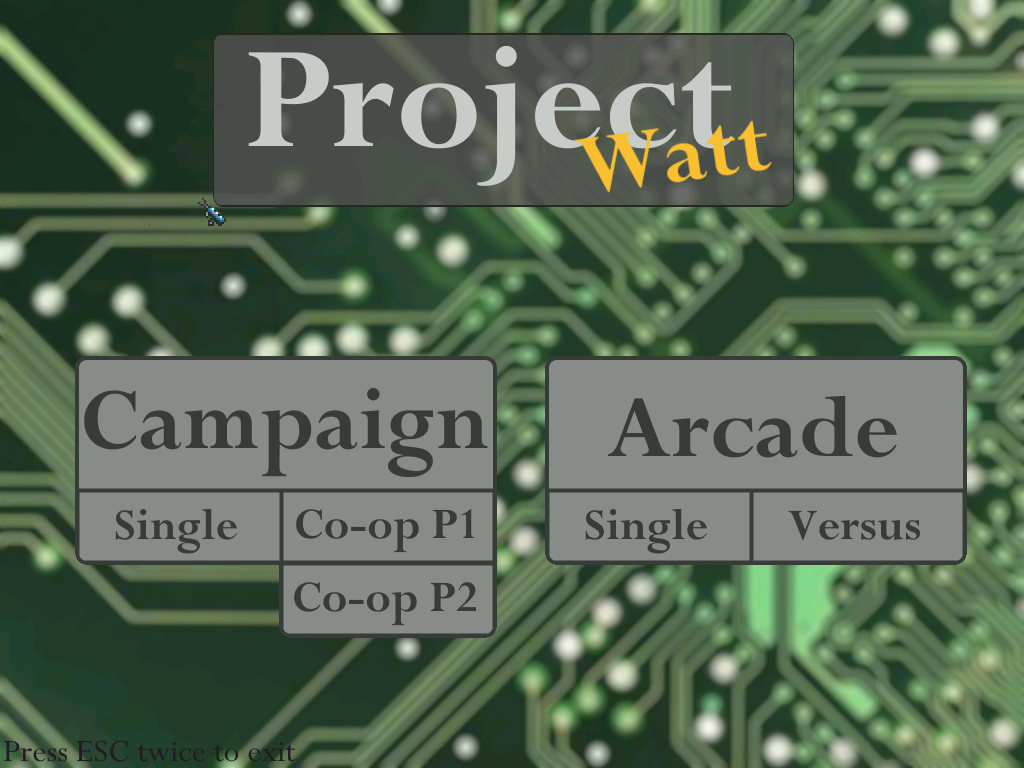
\includegraphics[width=\textwidth]{main_menu}

\section{Campaign}

Este é o modo de jogo \textit{principal} em que um jogador controla a personagem \textit{Watt}, uma faísca que ficou "presa" num curto-circuito e que para sair terá de fazer "ligação à terra", ou seja, neste caso, a personagem tem de alcançar o canto superior direito do mapa. Para isso tem de ultrapassar diversos obstáculos tais como os espinhos e lasers (se tocar num destes a faísca dissipa-se e volta ao início). \newline
O movimento da personagem principal é controlado pelas teclas W, A, S, D ou pelas setas $\uparrow$, $\leftarrow$, $\downarrow$ e $\rightarrow$ e o seu salto pela tecla Z ou pelo Espaço.
Para além disso, é possível controlar certos aspetos da jogabilidade, como a altura do salto da personagem e a sua velocidade (através dos \textit{sliders} azul e laranja respetivamente), qual dos lasers está inativo (vermelho, azul ou roxo - através dos botões com a cor correspondente) e o sentido da gravidade da personagem (através da tecla X em multiplayer, uma knob em Co-Op). Todos estes aspetos são controlados pelo segundo jogador se estiver a jogar em Co-Op.

% \includegraphics[width=\textwidth]{singleplayer}

\section{Arcade}

Um modo de jogo alternativo, baseado na mecânica de anti-gravidade do outro modo de jogo, em que o jogador terá de se desviar de lasers que vêm na sua direção, passando por entre estes e tentanto aguentar o máximo de tempo possível sem tocar neles e perder.

% 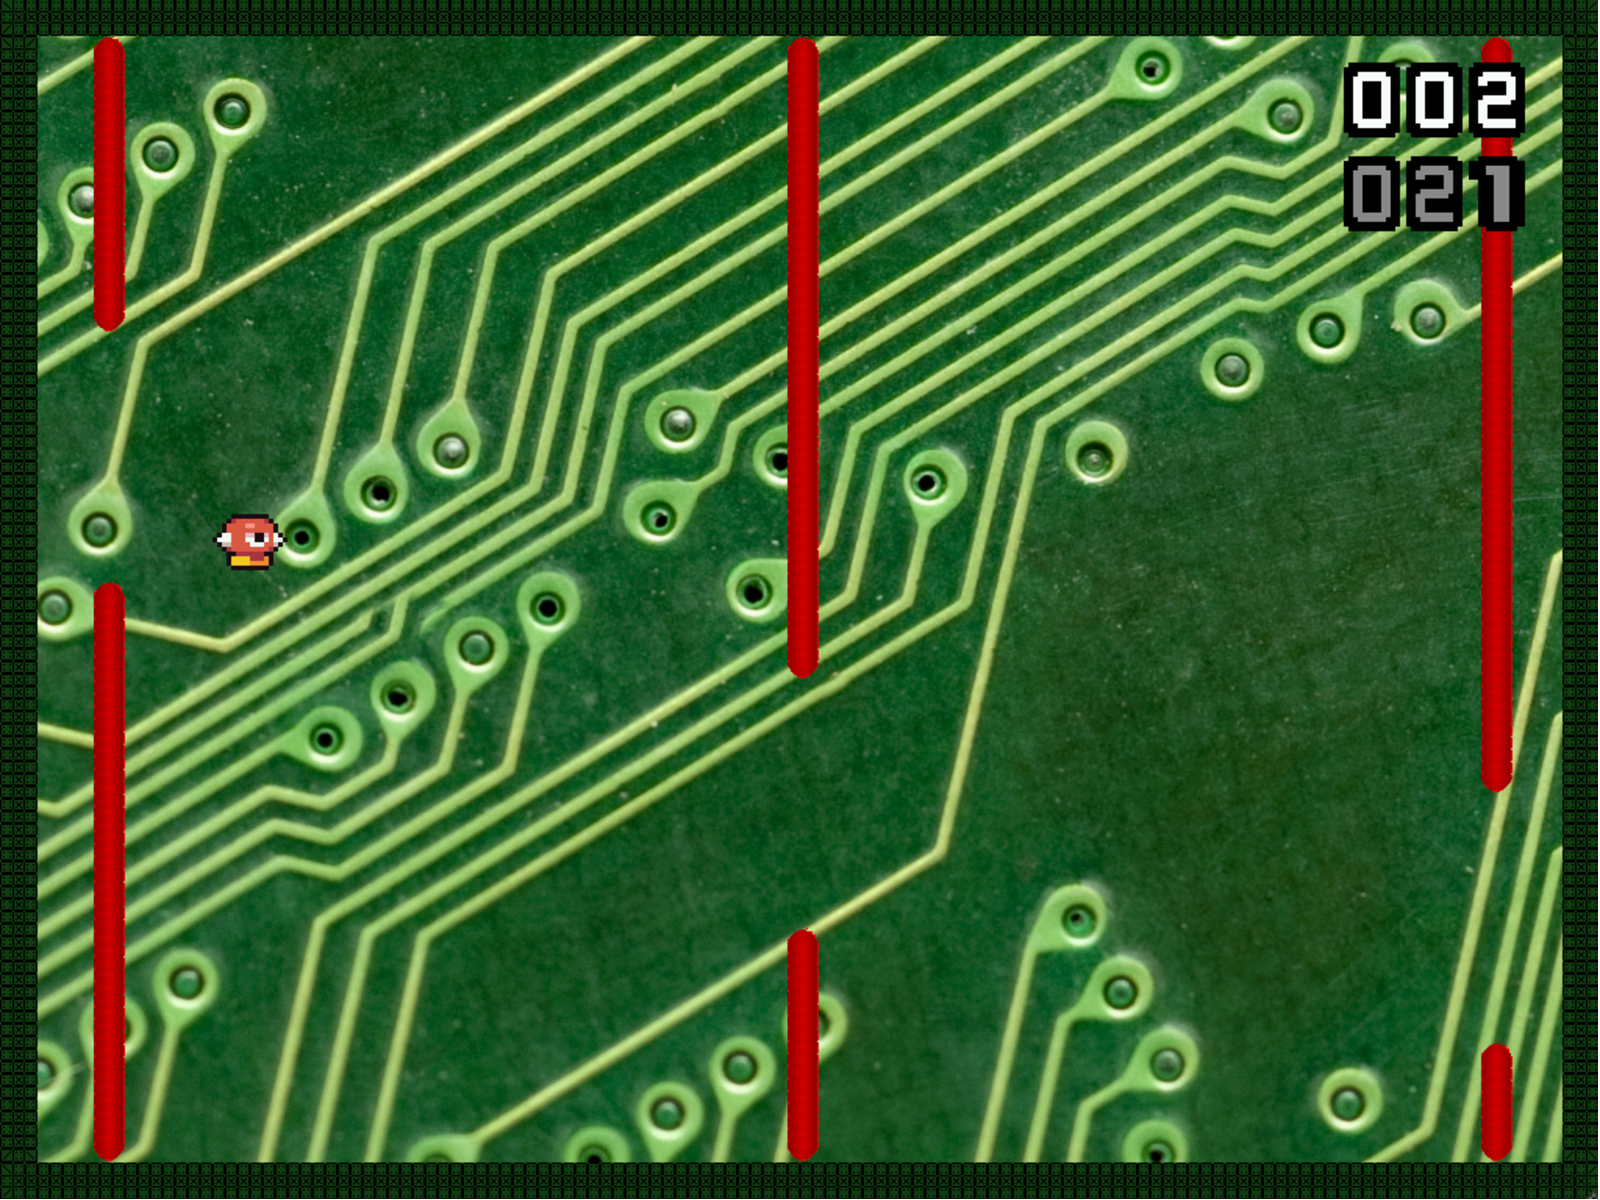
\includegraphics[width=\textwidth]{arcade}

\chapter{Estado do Projeto}

\section{Dispositivos Usados}

\begin{center}
	\begin{tabular}{|c|c|c|} 
		\hline
			Dispositivo & Utilização & Interrupção \\ 
		\hline
		\hline
			Timer & N/A & Sim \\ 
			Teclado & Controlo da personagem 1 & Sim \\ 
			Rato & Menus e personagem 2 & Sim\\
			Placa Gráfica & Desenho dos menus e do jogo & Não\\
			Real Time Clock & Efeito temporário & Sim\\
			Serial Port & N/A & Sim \\
		\hline
	\end{tabular}
\end{center}

\subsection{Timer}

Framerate handling

\subsection{Teclado}

\subsection{Rato}

\paragraph{}
Usado no menu principal para selecionar o modo de jogo e para controlar sliders/knob.

\subsection{Placa Gráfica}

\paragraph{}
RGB 565

\subsection{Real Time Clock}

\subsection{Serial Port}

\paragraph{}
Usado nos modos multiplayer (Campaign - Co-Op e Arcade - Versus). No primeiro, as personagens 1 e 2 são controladas pelos utilizadores em máquinas separadas, sendo que estas interegam entre si do seguinte modo: A personagem 2 consegue inicialmente controlar tanto a velocidade como altura do salto da personagem 1,
porém, após esta obter certos powerups, a personagem 2 é notificada de que pode também controlar os lasers que estão ativos e o sentido da gravidade do jogador 1.

Feita com FIFOs

\chapter{Organização e Estrutura do Código}

\section{Geometry}

\paragraph{}
O módulo \textit{Geometry} é dividido em duas partes, \textit{Vec2d} e \textit{Rect}, e serve como base do nosso sistema de coordenadas, físicas, hitboxes e colisões.

\subsection{Vec2d}

\paragraph{}
Este módulo é usado para representar vetores de duas dimensões, e consequentemente, pontos no espaço. Cada \textit{vec2d} é composto pelas suas componentes horizontal (x) e vertical (y), seguindo o referencial do frame buffer (x no sentido da esquerda para a direita e y no sentido de cima para baixo).

Existe um conjunto de operações que podemos efetuar com esta classe, nomeadamente somar, subtrair, multiplicar por um escalar, a norma do vetor, o ângulo entre dois vetores (usado para a \textit{Knob}), produto escalar, a distância entre dois pontos do plano, calcular a posição de um ponto em coordenadas polares, entre outros (todas estas funções encontram-se expostas no Doxygen deste módulo).

\subsection{Rect}

\paragraph{}
Este módulo é usado para colisões e para o UI. 

\subsection{Sistema de Colisões}

\paragraph{}
Sistema de colisões.

\section{Bitmap}

\paragraph{}
O código que usamos ler bitmaps foi parcialmente retirado da internet, mas com várias alterações para melhor se ajustar ao tipo de \textit{bitmaps} que usamos (criados pelo GIMP).

Todos os ficheiros externos necessários (\textit{bitmaps}) encontram-se organizados dentro de uma pasta 'assets', cuja localização pode ser específicada ao iniciar o jogo (até um limite de 255 caracteres, incluindo os ficheiros no interior dessa pasta).

Com o intuito de reduzir a quantidade de \textit{bitmaps} criados, ao desenhar no ecrã cada \textit{bitmap} normal, existe a opção de o desenhar alinhado à esquerda, ao centro ou à direita do ponto do ecrã indicado num argumento. Para além desse argumento existe ainda a possibilidade de desenhar o simétrico de cada \textit{bitmap} segundo quer o seu eixo (centrado no \textit{bitmap}) horizontal, vertical ou ambos. Esta segunda \textit{feature} foi especialmente útil e importante para as animações do jogador. 

Ao desenvolver o projeto considerámos necessário uma maneira de poder renderizar todas as nossas plataformas, paredes, espinhos e lasers de uma maneira mais dinânmica, para evitar criar uma nova sprite manualmente por cada objeto novo dessas classes. Assim implementamos uma função bitmap\_draw\_dynamic() que nos permite criar \textit{bitmaps} bastante reduzidos e que ocupam extremamente pouca memória RAM. Cada um destes \textit{bitmaps} pode ser subdividido em 9 quadrados, todos de tamanho igual, específico de cada imagem. A função irá depois reproduzir cada secção apropriadamente para produzir no ecrã uma imagem do tamanho pretendido.

Existe ainda a possibilidade de cada pixel ser 'multiplicado' por uma cor. Devido ao custo pesado de computação desta operação, decidimos que usar uma operação bitwise entre a cor do pixel e da cor a multiplicar, visto que o efeito que ela produz seja satisfatório o suficiente para as nossas necessidades, mantendo um baixo custo computacional. Esta operação irá sempre escurecer a cor do \textit{bitmap} original, e quando aplicado a um pixel branco irá ficar apenas a cor a multiplicar. Esta propriedade foi usada a renderizar todas as plataformas e paredes. 

Todos os \textit{bitmaps} podem ser desenhados com 'transparência', isto é, definimos a cor rosa, 0xFF00FF (em RBG 888), como a cor que será sempre ignorada ao desenhar.

\section{Sprite}

\paragraph{}
No nosso programa existe duas classes de \textit{sprite}: a normal e a dinâmica. A dinâmica é usada sempre que quisermos usar a função bitmap\_draw\_dynamic() referida acima, a normal é usada em todos os outros casos.

Foi tomada a decisão de implementar as animações seguindo o popular \textit{Unity}. Este \textit{game engine} tem uma propriedade \textit{Animator} que pode ser acoplado a qualquer objeto com um \textit{Renderer}. O \textit{Animator} é apenas uma máquina de estados que indica, no momento de renderizar o objeto no ecrã, qual a \textit{Sprite}, textura ou \textit{3D Model} a usar.

O sistema que decidimos implementar está imbutido diretamente na nossa classe \textit{Sprite}, que permite criar cada objeto com até 255 \textit{bitmaps}. Para permitir a instanciação de tantos \textit{bitmaps}, recorremos a um construtor que aceita um número variável de argumentos. A nossa classe tem uma propriedade "estado da animação", que indica qual dos n \textit{bitmaps} a desenhar. Este estado pode obtido e alterado através de um par de setters e getters.

A máquina de estados responsável por controlar qual o valor deste estado (por \textit{default} este valor é 0, ou seja, o primeiro \textit{bitmap}). Este tema será abordado novamente ao discutir o \textit{player}.

Cada \textit{sprite} criada também tem um \textit{offset} individual que é utilizado ao renderizar o \textit{bitmap} no ecrã. Existe ainda um getter das \textit{sprites} (\textbf{Vec2d\_t sprite\_get\_size(Sprite\_t *s)})que permite obter o tamanho do primeiro \textit{bitmap} carregado, especialmente útil para obter dinâmicamente a \textit{hitbox} do \textit{player} e dos botões. 

\section{Game Manager}

\section{Hardware Manager}

\paragraph{}
Este módulo foi uma tentativa de tentar encapsular ao máximo todo o conhecimento e funções responáveis por interagir com o hardware num único sítio o e transparecer o mínimo possível sobre as nossas implementações internas do \textit{timer}, \textit{keyboard}, \textit{mouse}, etc..

Infelizmente existem outros módulos com um grande conhecimento destes protocolos, como o \textit{InputEvents}, o \textit{GameManager} e tudo o que envolvesse o \textit{serial port}.

\section{Timer}

Lab2

\section{Keyboard}

\paragraph{}
Para guardar o input do \textit{keyboard} recorremos à classe \textit{KbdInputEvents}, que mantém um registo sobre todos os \textit{scancodes} de 1 \textit{byte} e sobre um subset específico de \textit{scandodes} de 2 \textit{bytes}.

Com o propósito de criar um \textit{dispatcher} eficiente, foi usado um \textit{map} para mapear cada \textit{scancode} ao seu valor respetivo. É registada sempre se uma tecla está a ser pressionada e se uma tecla foi pressionada durante este frame (isto é, se o utilizador empurrou para baixo a tecla).

A função \textbf{kbd\_input\_events\_process\_scancode()} trata de interpretar qualquer scancode que seja recebido do \textit{keyboard}.

Para mais permito um acesso mais simples a estas informações a partir de qualquer ponto do programa, esta classe foi tornada um \textit{singleton}, com dois getters para saber se uma tecla se encontra premida, \textbf{get\_key(KeyboardMap\_t map)}, e se uma tecla foi premida neste frame, \textbf{get\_key\_down(KeyboardMap\_t map)}.

O \textit{KeyboardMap} utilizado como argumento é um \textit{enum} com todas as teclas suportadas. Isto também permite que se o layout do teclado for diferente do \textit{default}, os scancodes podem ser alterados apenas nesse \textit{enum}.

Para detetar se uma tecla foi premida num certo frame, foi necessário limpar esse segundo map no final de cada frame, isto é, após a chamada da função \textit{update()}, para garantir que os inputs são interpretados corretamente, recorrendo à função \textbf{reset\_kbd\_input\_state()}.

\section{Mouse}

\paragraph{}
Para abordar completamente o uso mais direto do \textit{Mouse} é necessário cobrir duas partes, o \textit{MouseInputEvents} e o \textit{MouseCursor}, sendo que o segundo tira partido do primeiro.
Tal como o \textit{KbdInputEvents}, estas duas classes são também \textit{singletons}.

\subsection{MouseInputEvents}

\paragraph{}
Esta classe guarda e expõe para o resto do programa os botões premidos pelo utilizador, se eles estão a ser premidos neste instante e se eles começaram a ser pressionados neste frame. Regista também o \textit{delta} do movimento do rato no eixo do x e y em cada frame.

Para permitir saber se um dado botão começou a ser premido num determinado frame e para garantir que o \textit{delta} do rato entre frames é o correto, recorremos ao mesmo truque do \textit{KbdInputEvents}, utilizando a função \textbf{reset\_mouse\_input\_state()}.

\subsection{MouseCursor}

\paragraph{}


\section{Video}

Lab5

\section{Level}

\section{Player}

\section{RTC}

O módulo do RTC é responsável por obter informação acerca da hora atual, bem como programar alarmes.

\section{UI Elements}

\section{Switchboard}

\section{Powerup}

\section{Proj}

\section{Call Graph}

\chapter{Detalhes de Implementação}

\chapter{Conclusões}

\end{document}